\section{Filteroperationen}
Bei Filteroperationen werden neu auch die Werte der Nachbarpixel in Betracht gezogen.\\
Es gibt folgende Filtertypen:
\begin{description}
    \item[homogene Filter] Die Berechnung der Transformation $f(g)$ wird für jedes Pixel unabhängig von dessen Position vorgenommen.
    \item[inhomogene Filter] Die Berechnung der Transformation $f(g)$ hängt explizit von der Position des Pixels im Bild ab.
    \item[lineare Filter] Die Berechnung der Transformation $f(g)$ hängt für jedes Pixel linear von $g=I_{m,n}$ und den Werten der Nachbarpixel $I_{p,q}$ ab.
    \item [nicht lineare Filter] Identisch mit den linearen Filtern, aber die Abhängigkeit zu den Pixeln ist nicht linear.
\end{description}

\subsection{Lineare Filter}
Lineare Filter werden durch eine Faltung (\ref{eq:conv}) oder Korrelation(\ref{eq:corr}) angewendet.
\begin{equation} \label{eq:conv}
I \otimes h: I_{m,n} \to \sum_{p=-u}^{u}\sum_{q=-v}^{v}I_{m-p,n-q} * h_{p,q}
\end{equation}
\begin{equation} \label{eq:corr}
I \otimes h: I_{m,n} \to \sum_{p=-u}^{u}\sum_{q=-v}^{v}I_{m+p,n+q} * h_{p,q}
\end{equation}
\subsubsection{Tiefpass (Glättung)}
Beim Glätten von Bildern wird durch eine Mittlung der Nachbarpixeln erreicht.\\
Bsp: $R=\frac{1}{9}*\begin{bmatrix}
1 & 1 & 1 \\
1 & 1 & 1 \\
1 & 1 & 1
\end{bmatrix}$
oder $G=\frac{1}{16}*\begin{bmatrix}
1 & 2 & 1 \\
2 & 4 & 2 \\
1 & 2 & 1
\end{bmatrix}$
\begin{lstlisting}
%apply a filter of size 2x2
R = 1/4*[1 1; 1 1];
Image1 = uint8(imfilter(double(Image), R));
\end{lstlisting}
\subsubsection{Hochpass (Kantenhervorhebung)}
Bei der Kantenhervorhebung werden Abweichungen zu den benachbarten Pixel signalisiert.\\
Dafür wird die Ableitung der Pixel eruiert (Herleitung Skript S.37).
\begin{equation}
\frac{\partial I}{\partial x}=\frac{I_{m,n+1}-I_{m,n-1}}{2} \to h_x = \frac{1}{2}*
\begin{bmatrix}
-1 & 0 & 1
\end{bmatrix}
\end{equation}
\begin{equation}
\frac{\partial I}{\partial y}=\frac{I_{m+1,n}-I_{m-1,n}}{2} \to h_y = \frac{1}{2}*
\begin{bmatrix}
-1 \\
0 \\
1
\end{bmatrix}
\end{equation}
Die obigen Filter $h_x$ und $h_y$ sind sehr fehleranfällig auf Bildrauschen. Durch die Faltung mit Glättungsfiltern kann dieses Rauschen aber reduziert werden.\\
Dies führt zu den Sobel und Prewitt Filter:
\begin{equation*}
Prewitt-Filter: h_x = \begin{bmatrix}
-1 & 0 & 1 \\
-1 & 0 & 1 \\
-1 & 0 & 1
\end{bmatrix}
h_y = \begin{bmatrix}
-1 & -1 & -1 \\
0 & 0 & 0 \\
1 & 1 & 1
\end{bmatrix}
\end{equation*}
\begin{equation*}
Sobel-Filter: h_x = \begin{bmatrix}
-1 & 0 & 1 \\
-2 & 0 & 2 \\
-1 & 0 & 1
\end{bmatrix}
h_y = \begin{bmatrix}
-1 & -2 & -1 \\
0 & 0 & 0 \\
1 & 2 & 1
\end{bmatrix}
\end{equation*}
\begin{lstlisting}
% Prewitt Filter
DX = [-1 0 1; -1 0 1; -1 0 1];
DY = DX';	
%apply the DX and DY filter
ImageDx = imfilter(Image, DX);
ImageDy = imfilter(Image, DY);
\end{lstlisting}
oder mit den Matlab Funktionen:
\begin{lstlisting}
%choose the filters
DX = fspecial('sobel')';
DY = fspecial('sobel');
%bzw
DX = fspecial('prewitt')';
DY = fspecial('prewitt');
%apply the DX and DY filter
ImageDx = imfilter(Image, DX);
ImageDy = imfilter(Image, DY);
\end{lstlisting}
\subsubsection{Bestimmen des Steigungswinkel}
Durch Trigonometrie kann die Richtung/Winkel der Steigung evaluiert werden.
\begin{equation}
\alpha = \arctan{\frac{\frac{\partial I}{\partial y}}{\frac{\partial I}{\partial x}}}
\end{equation}
\begin{lstlisting}
%determine the angle
%(atan2 gives back the whole interval
%]-pi , pi[ )
Angle = atan2(ImageDy, ImageDx);
\end{lstlisting}
\subsubsection{Bildschärfung}
Um ein Bild zu schärfen kann der Laplace Operator verwendet werden. Dieser ist als Summe der zweiten Ableitungen definiert (Herleitung Skript S 38):
\begin{equation}
\Delta I = L = \frac{\partial ^2I}{\partial x^2} + \frac{\partial ^2I}{\partial x^2} \to L = \begin{bmatrix}
0 & -1 & 0 \\
-1 & 4 & -1 \\
0 & -1 & 0
\end{bmatrix}
\end{equation}
In der Bildverarbeitung wird der Laplace Operator wie folgt eingesetzt:
\begin{equation}
1*I+\beta * L
\end{equation}
Wobei der Term $1*I$ benötigt wird, damit das Bild in die Berechnung hineingezogen wird (L alleine detektiert nur die Kanten). Der Faktor $\beta$ beschreibt wie stark das Bild geschärft werden soll.
\begin{lstlisting}
%define the filter
Beta = 0.5;
Mask = [0 0 0; 0 1 0; 0 0 0] + Beta*[0 -1 0; -1 4 -1; 0 -1 0]
%apply the filter
ImageEnh = imfilter(Image, Mask);
\end{lstlisting}

\subsection{Nichtlineare Filter}
\subsubsection{Median Filter}
Der Median-Filter hilft beim entfernen von Bildstörungen oder beim finden von lokalen Maximas und Minimas.
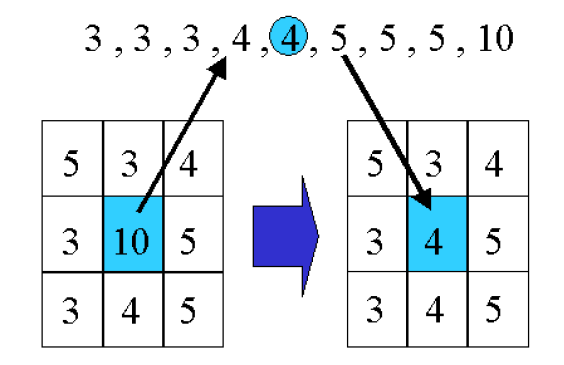
\includegraphics[width=\textwidth/3]{medianfilter.PNG}
\begin{lstlisting}
% 5 means take the 5th element in the value order
ImageMedian = ordfilt2(ImageNoise, 5, ones(3,3));
\end{lstlisting}
\subsubsection{Minimas und Maximas}
\begin{lstlisting}
%apply min/max filter
MinVal = ordfilt2(ImgValley, 1, ones(SizeRegion));
MaxVal = ordfilt2(ImgHill, SizeRegion^2, ones(SizeRegion));

%find local min/max values
LocMin = (MinVal == ImgValley);
LocMax = (MaxVal == ImgHill);
\end{lstlisting}
